\chapter{国内外相关研究现状}\label{chap:related_work}

目前,国内外针对从非结构化文本中进行需求发现和提取已经有一些论文成果。在许多开源和工业项目中,开发人员大量使用书面沟通渠道,例如邮件列表,issue tracker、聊天工具等,并且这样的方式已经遍布全球开发人员的日产工作中。自然语言处理技术和文本挖掘如情感分析、话题建模、机器学习等技术首先被应用于这些文本的意图分类中,如缺陷报告分类、特征请求分类等\cite{maalej2015bug},并且服务于发布计划工具,向应用开发者提供支持,决定哪些新特征需要在下个版本中实现。本文主要从特征请求对话识别工具构建过程中所涉及的相关概念以及技术细节包括基于文本数据的需求发现、聊天对话文本在软件工程中的应用、对话解耦、文本表示和文本分类以及少样本学习几方面进行探究并介绍国内外相关研究工作。

\section{基于文本数据的需求发现}


目前,人工和自动分析比如基于规则的方法以及有监督的机器学习方法正在被大量应用在分析对软件工程师和非技术利益相关者有用的如特征请求等信息中\cite{Morales2019Speech},并已有大量相关的研究工作。
\subsection{基于手工规则的需求发现}

RE Vlas等人\cite{morales2014discovering}提出一种基于语法的特征请求发现工具。作者使用Subject-Action-Object(SAO)语法标签对需求进行解析和表示。其中subject是需求声明的发出者,action定义了需求里面定义的特征,object表示被action影响的对象。比如:“这个提交按钮应该把表单数据提交给处理组件”中,“提交按钮”是subject,“发送”是action,object是“表单数据”。图\ref{fig:sao}是SAO方法对密码安全特征需求进行识别的一个例子。
\begin{figure}[htbp]
    \centering
    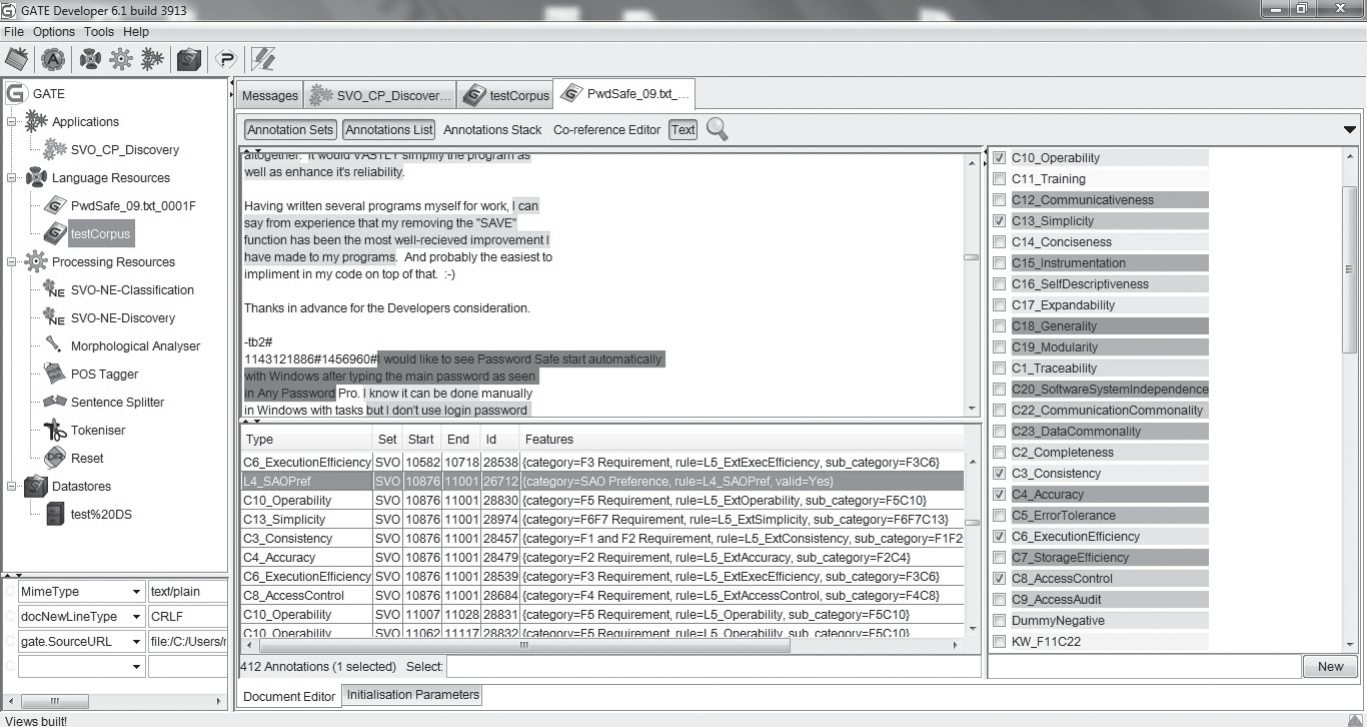
\includegraphics[width=0.70\textwidth]{Img/sao.png}
    \bicaption{基于SAO方法对密码安全特征需求进行识别}{SAO-based Recognized Password Safe Feature Requirements}
    \label{fig:sao}
\end{figure}


邮件是开发者之间进行沟通的重要方式之一,通常包含特征请求、观点询问、问题发现、解决方案、信息提供等不同类别的信息。Di Sorbo等人\cite{Sorbo2016Development}提出一种名叫DECA(开发者电子邮件内容分析器)的半监督学习方法,通过使用自然语言解析工具分析文本的语言学特征并且从询问帮助、提供帮助、提出新需求、报告或者讨论BUG等几方面对开发者的意图进行分类。Di Sorbo等人首先根据来自Ubuntu和QT的数据设置更适合邮件列表信息的分类,具体分类类别如表\ref{tab:deca0}所示。
\begin{table}[htb]
\bicaption{句子例子以及对应的类别}{Sentence examples and corresponding categories}
    \label{tab:deca0}
    \centering
    \footnotesize% fontsize
    \setlength{\tabcolsep}{4pt}% column separation
    \renewcommand{\arraystretch}{1.2}%row space 
\begin{tabular}{lcccccccc}
\hline
句子类别的例子      & 分类类别 \\
\hline
讨论一个变更       & 特征请求 \\
定位BUG        & 问题发现 \\
BUG是否被修复     & 信息询问 \\
针对已知问题提出解决方案 & 解决方案 \\
请求其他开发者做出变更  & 特征请求 \\
询问代码时如何工作的   & 信息询问 \\
询问为何这样写代码    & 信息询问 \\
向某人征求意见      & 意见询问 \\
找出代码作者       & 信息询问 \\
更多的了解代码      & 信息询问 \\
告诉其他开发者一些事情  & 信息提供 \\
\hline
\end{tabular}
\end{table}
然后对其进行手工标注,作者发现开发人员在关于开发问题的讨论中撰写关于现有错误或者建议提出特征请求时,他们倾向于使用一些经常性的语言模式,比如对于“我们可以使用漏桶算法来限制带宽”,可以发现句子中提供一个明确定义的谓词-参数结构,对此,可以看出大多数具有谓词-论元结构的句子表明解决方案。作者定义了启发式规则,首先发现句子的特定句法结构,然后推广某些类型的信息,最后忽略无用的信息。所以,作者定义了“【某人】可以使用【某事物】”的一般模式来识别解决方案。图\ref{fig:deca1}是作者通过斯坦福依存句法分析来分析启发式规则时的例子。
\begin{figure}[htb]
    \centering
    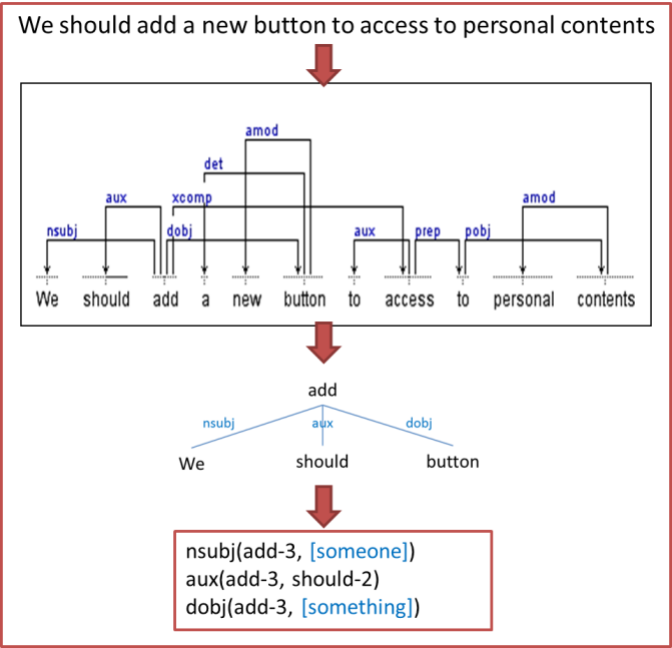
\includegraphics[width=0.60\textwidth]{deca1}
    \bicaption{特征请求中的自然语言解析树}{Natural language parsing tree about feature request}
    \label{fig:deca1}
\end{figure}
作者通过图\ref{fig:deca1}定义了“【某人】应添加【某事物】”的启发规则并于特征请求相关联。Andrea Di Sorbo等人的观点是在软件工程领域始背相关的重复语言模式,这对软件过程中的需求分析非常有用。

L Shi等人\cite{shi2017understanding}提出利用自然语言处理技术生成一组模糊规则来自动分析和构造特征请求的方法,将特征请求中的每个句子进行分类,类别有意图、解释、益处、缺点、示例和无关,分类的结果用来增量生成模糊规则。作者定义了这些类别以及类别的定义和优先级来帮助构建特征请求并突出显示值得关注的内容,如表\ref{tab:fra0}所示。
\begin{table}[htb]
\bicaption{句子类别的定义}{Definitions of sentence categories}
    \label{tab:fra0}
    \centering
    \footnotesize% fontsize
    \setlength{\tabcolsep}{4pt}% column separation
    \renewcommand{\arraystretch}{1.2}%row space 
\begin{tabular}{lcccccccc}
\hline
类别 & 重要性 & 定义                     \\
\hline
意图 & 1   & 关于改进系统和功能的主意、需求、期望的描述  \\
益处 & 2   & 关于提出的需求带来的好处和有帮助的结果的描述 \\
缺点 & 3   & 关于当前系统行为的缺点            \\
例子 & 4   & 关于支持提出的需求的例子           \\
解释 & 5   & 关于提出需求的场景和解决           \\
无关 & 6   & 和系统无关的信息              \\
\hline
\end{tabular}
\end{table}
作者分别在词汇、语法、语义三个级别启发式地定义模糊规则。词汇通过设置不同类别的词汇表来设置不同句子类别的模式,句法通过对句子进行依存结构分析不同句子类别的句法特征,语义层面通过定义在某个类别的句子中中的语言表达的含义,如图\ref{fig:fra1}所示的语义模式。
\begin{figure}[htb]
    \centering
    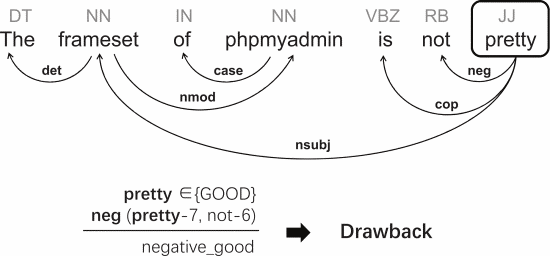
\includegraphics[width=0.70\textwidth]{fra1}
    \bicaption{缺陷类别的语义模式示例}{An example about semantic pattern of defect class}
    \label{fig:fra1}
\end{figure}
实验表明,随着新规则的引入,模糊规则的分类性能越来越高。此外,在将模糊规则转换成布尔变量之后,将其应用于各种机器学习算法上得到了更好的效果。

I Morales-Ramirez等人\cite{Morales2019Speech}关注于分析在线讨论,如开源软件的邮件列表和用户论坛,在这里,不同的利益相关者比如开发者、软件终端用户会讨论有助于软件发展的信息。基于规则Speech-acts分析\cite{morales2014discovering}用在线讨论的自动分析上,比如,通过学生的查询理解学生的意图\cite{feng2006intelligent}等。 Speech-acts理论认为当某人说一些话让对方相信或者做出对应的行为\cite{acts1969essay}。比如在询问一个新特征中使用的词汇包括:“添加特征”、“想要这个特征”等。作者把不同speech-acts规则归为几类:c-Assertive, c-Responsive, c-Requestive和c-Attachment。如表\ref{tab:speech-act0}所示,每一列为对应的独立speech-acts类别。
\begin{table}[htb]
\bicaption{Speech-acts列表}{List of speech-acts}
    \label{tab:speech-act0}
    \centering
    \footnotesize% fontsize
    \setlength{\tabcolsep}{4pt}% column separation
    \renewcommand{\arraystretch}{1.2}%row space 
\begin{tabular}{lcccccccc}
\hline
c-Assertive & c-Requestive & c-Responsive & c-Attachment & c-Other          \\
\hline
断定        & 请求         & 回应         & 附件         & 描述性的      \\
确认        & 需求         & 建议         & 代码         & 接受           \\
让步        & 问题         & 支持         & URL链接      & 拒绝           \\
            &              &              & 日志文件     & 消极观点 \\
            &              &              &              & 积极观点  \\
            &              &              &              & 感谢            \\
            &              &              &              & 内容丰富的 \\
\hline            
\end{tabular}
\end{table}
基于Speech-acts的模型结构如图\ref{fig:speech-acts1}所示。
\begin{figure}[htb]
    \centering
    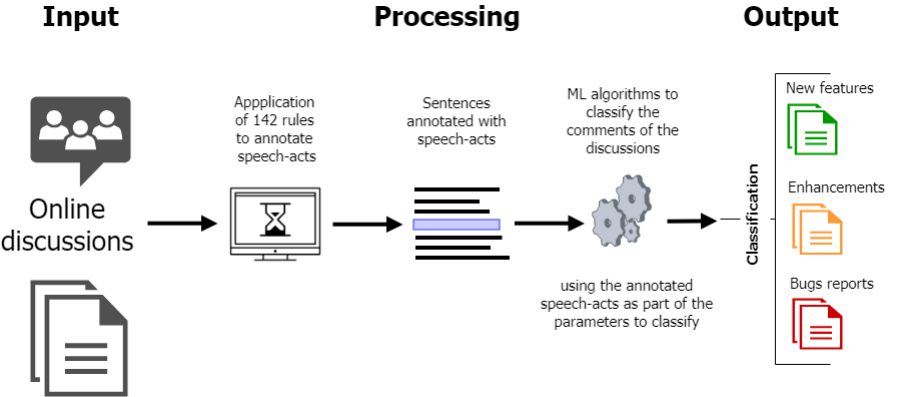
\includegraphics[width=0.70\textwidth]{Img/speech-acts1.png}
    \bicaption{基于Speech-acts的分析模型}{Speech-acts based analysis approach}
    \label{fig:speech-acts1}
\end{figure}
这个工具结合了作者基于他们关于需求的知识以及利益相关者在在线讨论中表达他们需求的方式定义的142条词法-句法规则,从而对特征请求进行发现。

\subsection{基于统计机器学习的需求发现}
开发者和客户通常会通过会面来获取用户故事,P Rodeghero等人\cite{Rodeghero2017Detecting}提出一种从客户和开发人员之间记录的对话中自动提取和用户故事相关的信息。作者从开发人员和客户之间的对话记录中自动提取用于编写用户故事的数据,分别进行定性研究,以检验开发者和客户之间的对话包含用户故事的角色、功能和基本原理的假设,以及定量研究以确定现有分类算法的效果。作者通过定性研究分析得到大约5.5\%的对话包含功能信息,2.9\%包含了基本原理,只有0.5\%讨论了角色,发现对话包含重要的功能和基本原理信息,但关于角色的数据非常有限。作者训练了一个分类器用于检测包含功能数据的对话部分。在数据收集部分,作者收集一家软件开发公司的会议记录,并标注文件名、会话、摘要、会话转折、角色、功能、理由等信息,作者提取了25个属性进行分类,并且分析的单位是转折而不是句子,提出的方法模型如图\ref{fig:Rodeghero2017Detecting}所示。
\begin{figure}[htb]
    \centering
    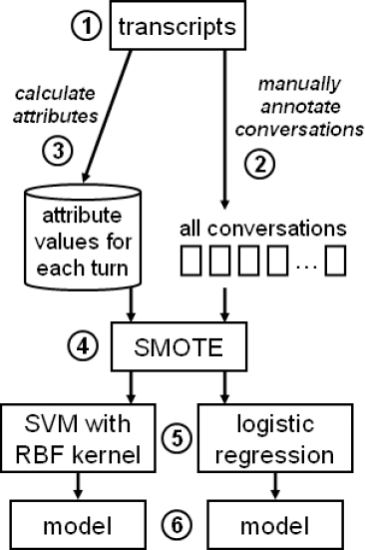
\includegraphics[width=0.40\textwidth]{Rodeghero2017Detecting.png}
    \bicaption{分类器模型结构图}{Structure of classifier}
    \label{fig:Rodeghero2017Detecting}
\end{figure}

Q Huang等人\cite{Huang2018Automating}发现Di Sorbo等人的分类类别还有55\%的句子不能覆盖,于是在其分类的基础上合并了两种意图,并新增了两种意图,提炼过的分类类别如表\ref{tab:aim0}所示。
\begin{table}[htb]
\bicaption{精炼后的意图分类}{Intention classification after refine}
    \label{tab:aim0}
    \centering
    \footnotesize% fontsize
    \setlength{\tabcolsep}{4pt}% column separation
    \renewcommand{\arraystretch}{1.2}%row space 
\begin{tabular}{lcccccccc}
\hline
类别   & 描述                 \\
\hline
信息提供 & 将知识、经验、计划、更新共享给其他人 \\
信息寻找 & 希望得到信息和帮助          \\
特征请求 & 帮助改进现有功能或提出新功能     \\
解决方案 & 共享可能的解决方案          \\
问题发现 & 报告BUG,或描述异常行为      \\
侧面评价 & 表达观点或进行评价          \\
无意义  & 无意义的或不重要的         \\
\hline
\end{tabular}
\end{table}
并提出了使用Convolutional Neural Network(CNN)\cite{kim2014convolutional}的方法自动将句子分类为不同的意图类别,整体模型架构如图\ref{fig:aim1}所示。
\begin{figure}[htb]
    \centering
    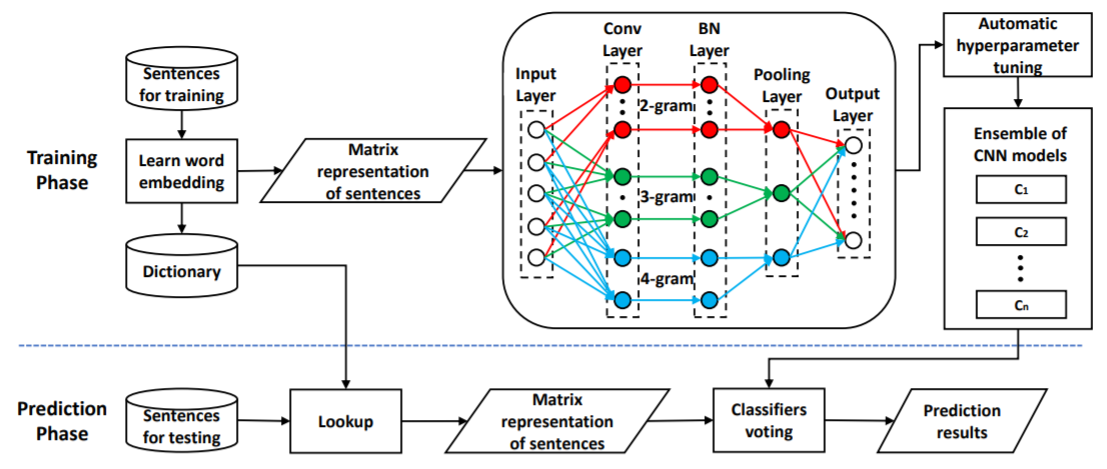
\includegraphics[width=0.8\textwidth]{aim1.png}
    \bicaption{CNN分类模型整体框架}{Structure of CNN classifier}
    \label{fig:aim1}
\end{figure}
CNN将句子作为输入,输入7个概率值,从而得出概率最大的句子类别,即使测试集中没有出现和训练集相似的模式或者关键词,模型也会给出概率最大的类别,从而覆盖所有句子。

Y Zhang等人\cite{zhang2015sensitivity}发现词向量的维度、过滤器的数量以及过滤器的深度是影响较大的超参数,作者使用贪婪的方式搜索最优参数。
D Arya等人\cite{arya2019analysis}通过对15个问题讨论进行内容定量分析确定包括潜在特征请求在内的16种信息类型。作者手工构建了14个对话特征,并使用随机森林作为分类器,对表达新特征请求的句子可以达到66\%的F1值。
W Maalej等人\cite{maalej2015bug}使用自然语言处理技术包括文本分类、情感分析把App Reviews分类为缺陷报告、特征请求、用户经验和打分。其中分类结果的precision可达到70-95\%,recall可达到80-90\%。
\section{聊天对话文本在软件工程中的应用}
在各种软件开发项目中,两种常见的聊天方式为同步和异步沟通方式\cite{yu2011communications}。同步方式包括Internet Relay Chat(IRC)等聊天工具,异步方式包括邮件列表、Issue tracker等工具。
基于Web平台的关于软件应用和服务的在线聊天讨论在包括需求发现等各种软件工程任务中表现出来巨大的价值\cite{Morales2019Speech},目前已有大量的研究工作正在开发有效的工具支持软件分析。它们利用自然语言处理技术从应用商店评论、在线聊天记录、邮件列表、用户论坛等文本数据中抽取相关信息,并且使用文本挖掘和机器学习技术对信息进行分类如缺陷报告或者特征请求。其中聊天记录中包含着关于软件系统的丰富的信息。

B Lin等人\cite{lin2016developers}通过一项关于开发者怎么使用Slack、哪个聊天工具在开源社区比较流行、聊天工具能够为软件开发带来怎么样的好处的研究,发现开发者使用Slack进行个人、团队、社区级别的交流,Slack也占据越来越重要的地位,在某些情况下会代替邮件。
E Shihab等人\cite{shihab2009studying}通过两个大型开源项目从几个维度分析了开发者IRC会议:会议内容、会议参与者、他们的贡献、会议类型。作者的研究表明IRC正在开源社区占据越来越重要的地位,强调了从开发者聊天记录中可以获取丰富的信息。
P Chatterjee等人\cite{chatterjee2019exploratory}调查了通过挖掘开发者谈话从而支持软件维护和演化的有效性和挑战性,作者发现开发者倾向于通过即时聊天工具分享对于观点或者有意义的想法,并且说明了通过应用一些技术和训练集可以达到较高的对话解耦效果。

\section{自然语言处理中的对话解耦}
聊天是开发者社区之间的一种同步文本通信方式。
当一组人在公共的聊天平台进行通信时,聊天中的消息形成流式信息,往往会有很多的对话同时出现,会话经常耦合在一起,例如单个会话会与其他会话交织在一起。并且如同 Internet Relay Chat(IRC)、Google Hangout、网站评论等聊天平台不能显式地表明对话的结构。将聊天消息划分为一组不同的对话是任何上层对话分析的基本前提。对话解耦就是从一个单一的流信息中识别独立对话的一个任务。

目前,关于对话解耦做出重要贡献的是一系列在IRC上标注的数据和训练的模型。
Adams和 Martell等人\cite{adams2008topic}研究了对话解耦和话题识别,但是没有公开数据集。Riou等人\cite{riou2015using}在IRC的\#Ubuntu-fr Channel标注对话以及句子关系。Lowe等人\cite{lasecki2013conversations}启发式地从\#Ubuntu Channel进行对话抽取。他们的工作提供了930,000个解耦的对话,为其他对话解耦工作提供了数据基础。
Elsner和Charniak等人\cite{elsner2008you}探索了使用信息对特征集和线性分类器,结合局部和全局的推断方法。Jiang等人\cite{jiang2018learning}使用了神经网络的方法,效果达到了提升。

JK Kummerfeld等人\cite{kummerfeld2018large}手工标注了一个大小为77,563条的解耦对话,对于对话定义了一个回复关系图模型,数据集包含内部的对话结构。如图\ref{fig:example-conversation}所示的两个耦合的对话和一个标注的图结构数据是标注数据集的一个样例,其中不同颜色的连线表示图连接。这个例子包括一个当多个人独立的尝试帮助BurgerMann时收到的多个回应的信息,并且在最后消息中BurgerMann回复多个信息。我们也可以看到delire和Seveas两个用户同时参与两个交谈中。
\begin{figure}[htb]
    \centering
    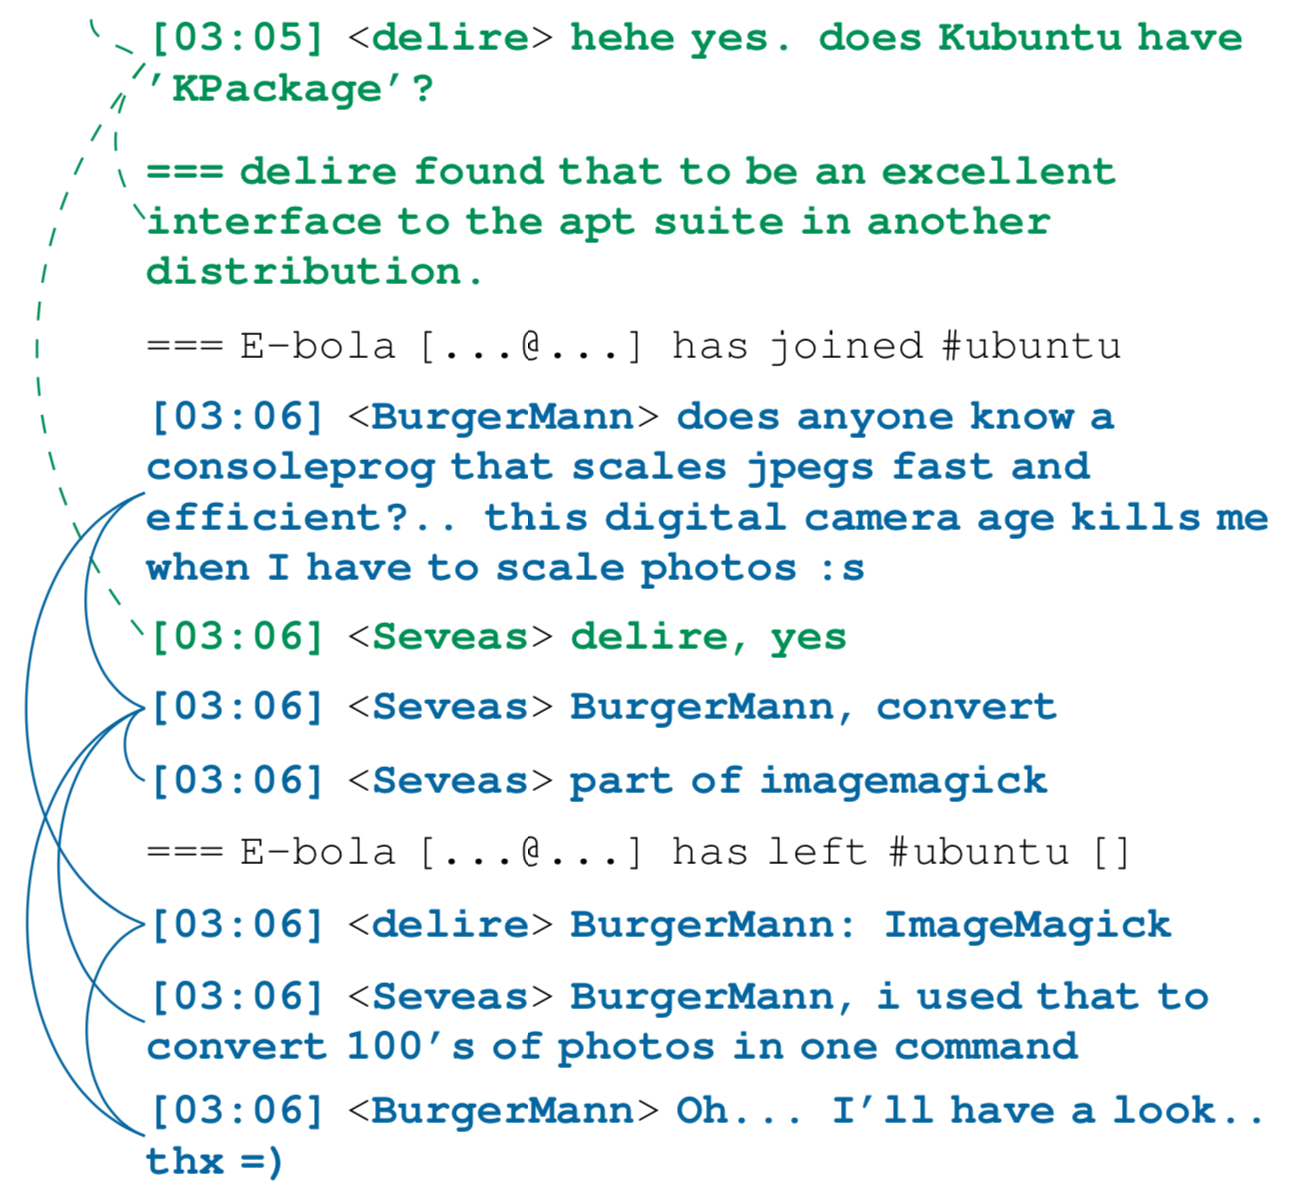
\includegraphics[width=0.6\textwidth]{Img/example-conversation.png}
    \bicaption{Ubuntu的例子。曲线是回复图结构的标注,其中蓝实线和绿虚线分别代表两个对话}{\#Ubuntu log sample. Curved lines are graph annotations of reply structure, which define two conversations shown with blue solid edges and green dashed edges}
    \label{fig:example-conversation}
\end{figure}
作者设计了一个具有2层、512维隐藏层和sigmod非线性激活函数的浅层前馈神经网络,并手工设计了77个特征,其中每个元素都是从原始对话文本中提取的数字类别特征,其中包括当前用户发布的先前聊天消息的时间间隔、聊天内容中是否有目标用户、两个聊天文本是否包含相同的单词等。该模型可以达到74.9%的精度和79.7%的召回率,具有相对较好的效果。

\section{自然语言文本的嵌入式表示和文本分类}
\subsection{TF-IDF}
探索如何基于稀疏或者稠密向量高效表示句子语义、语法信息是自然语言处理研究人员关注的一项工作。在现有各种文本向量表示方法中,TF-IDF(term frequency–inverse document frequency)\cite{chowdhury2010introduction}常用于信息检索与数据挖掘的加权技术,通过以词频、逆文档频率表示的词的重要性程度来表示句子。TF-IDF主要包含两部分:词频TF和逆文档频率IDF。其中,TF是词在文本中出现的次数,出现次数越多,表示该词越重要并在文本中占据重要的语义。对于词$t_i$来说其TF为,$tf_{i,j}=\frac{n_{i,j}}{\sum_k{n_{k,j}}}$,其中$n_{i,j}$代表该词在文档$d_j$中出现的次数,分母为在文档$d_j$中所有词出现的次数总和。
IDF是词出现在不同文档数的逆,词出现的次数越多,代表该词属于停用词如“的”、“是”、“了”等的概率越大。对于一个此来说,其IDF为$idf_{i}=\frac{|D|}{\{j:t_i \in d_j\}}$,其中$|D|$为文档总数,$\{j:t_i \in d_j\}$代表包含词$t_i$的文档总数,如果该词语不在语料库中,就会导致被除数为零,因此一般情况下使用$1+\{j:t_i \in d_j\}$。当有TF和IDF后,将这两个值相乘,也即$tfidf_{i,j}=tf_{i,j}\times idf_i$,就能得到一个词在文档集中的TF-IDF的值。在得到每个词的TFIDF后,对于文档集的词集合$V$,我们通常使用长度为$|V|$的向量表示文档,其中每个元素的值为出现在该文档的词的TFIDF值,没有出现则对应位置为零。然后,我们可以得到文档的向量化表示,继而运用到下游如文本分类、文本聚合等任务中。
\subsection{GloVe}
近来许多研究工作成功地通过学习词的向量空间表示如Word2Vec\cite{mikolov2013distributed}等来细粒度地获取语法和语义信息。这些向量可以被应用在各种任务上,如信息检索、文本分类、自动问答和命名实体识别等。词向量方法使用词对之间的距离或者角度作为评估词表示质量的主要方法。比如:“国王之于王后相当于男人之于女人”,其应该在向量空间表示为“国王-王后=男人-女人”。当前,主要有两种方式进行词向量学习:1)全局矩阵分解方法,如隐式语义分解(LSA)\cite{deerwester1990indexing}等,其使用矩阵的低秩近似将大矩阵进行分解,从而获取语料的统计信息。但是其问题在于高频词将会严重地影响相似度,然而它们是有很少的语义关联的;2)局部上下文窗口方法,如Skip-gram和CBOW方法\cite{mikolov2013distributed},但是其方法局限于只利用了窗口词,没有利用语料巨大的词共现信息。GloVe是一个无监督的获取词向量的算法,通过在聚集的全局词共现矩阵上进行训练,既使用了语料库的全局统计特征,也使用了局部的上下文特征,其结果显示了在词向量空间的线性特征。GloVe学习词向量的目标是学习词的共现概率比,如词$k$“固体”和词$i$“冰”共现的概率要比和词$j$“蒸汽”共现的概率大,则我们希望$\frac{P_{ik}}{P_{jk}}$尽可能大,其中$P_{ij}$是词$W_i$出现在词$W_j$上下文的概率。作者据此建立词向量模型:
$$F(w_i, w_j, w_k) = \frac{P_{ik}}{P_{jk}}$$
其中$w_i,w_j,w_k$分别为词$W_i,W_j,W_j$的词向量。为了保持词向量在线性空间的相似性,对模型进一步改进为:
$$exp(w_i^Tw_k-w_j^Tw_k)=\frac{P_{ik}}{P_{jk}}$$
为避免对称性带来的顺序不敏感性,对模型加入偏置项:
$$\log X_{ik}=w_{ik}+b_i+b_k$$
其中$X_{ik}$代表词$W_k$出现在词$W_i$上下文的次数。考虑到词共现的次数越多,这两个词对目标函数影响越大,因此根据词共现次数设计权重对目标函数进行加权:
$$J=\sum_{ik}X_{ik}(w_i^Tw_k+b_i+b_k-\log X_{ik})^2$$
GloVe模型产出了在线性词向量空间上有意义的结果,并达到了超越其他现有模型的效果,尤其在单词相似性比较任务上的表现非常出色。

\subsection{TextCNN}
聊天消息中的对话是按时间顺序记录的文本句子的形式,这是开发人员在在线交流中进行的。建模句子表达形式是高级对话分析的基础,在本文中,我们使用TextCNN\cite{kim2014convolutional}来表示句子,因为它使用简洁的网络结构和少量参数,因此在学习不充足的标记数据上具有优势。
TextCNN是用于句子建模的经典方法,它使用浅层卷积神经网络(CNN)\cite{krizhevsky2012imagenet}对句子表示进行建模。CNN是一种已广泛用于计算机视觉的深度学习模型。它使用几个卷积核捕获局部信息,然后使用这些局部信息生成全局表示。类似地,在自然语言处理(NLP)中,CNN可以聚合n元语法信息和建模句子表示形式。TextCNN将预训练或随机生成的单词嵌入作为输入,其输出的维数取决于卷积核的数量和大小。长度为$n$的句子可以表示为形状为$n\times d$的矩阵,其中$d$是单词嵌入的维数。每个内核为 $w \in \mathbb{R}^{kd}$ ,其中$k$是卷积内核的大小,应用于$k$个单词的窗口,然后映射到一个新的一维向量中。令$X_{i:i+k}$表示原始句子中的\textit{k}-gram单词串,然后对其进行卷积运算。卷积层的输出可以表示为$o_i=f(w\cdot X_{i:i+k} + b)$ ,其中$b$是偏置项,$f$是激活函数。给定一个句子的长度l和卷积核大小$k$,我们可以获得大小为$l-k+1$的句子的表示形式。卷积层后面是最大池化层,它可以捕获具有最大值的关键信息。
为了获得由不同尺度的局部信息组合而成的更充分的语义信息,我们可以将具有不同大小的多个卷积核应用于该句子。 因此,对于一个给定$n \times m$积核的句子,其中$n$是不同大小的核数,而$m$是每种大小的数量,我们可以得到大小为 $n\times m$的句子表示形式,其将不同尺度的局部信息转化为句子的整体表示。如图\ref{fig:textcnn}所示为TextCNN应用在句子分类上的模型结构图,其中不同颜色的矩阵为不同大小的二维卷积核,输出为二维向量用于句子分类。
\begin{figure}[htb]
    \centering
    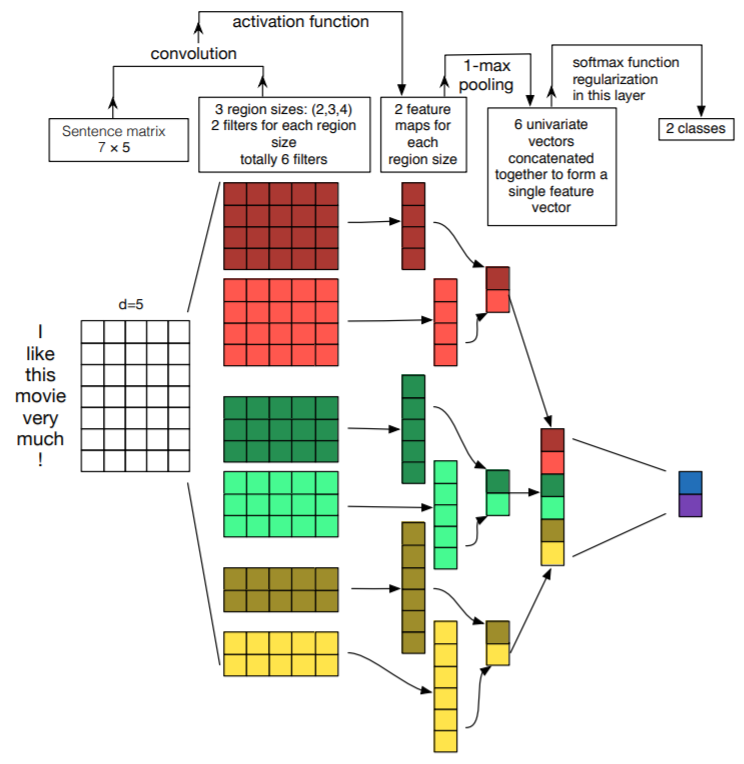
\includegraphics[width=0.6\textwidth]{Img/textcnn.png}
    \bicaption{一个用于句子分类的CNN结构表示。}{Illustration of a CNN architecture for sentence classification.}
    \label{fig:textcnn}
\end{figure}

\subsection{BiLSTM}
分析来自聊天消息的对话是一项上层的文本挖掘任务。因为当理解一个句子时,它需要考虑对话范围内的上下文信息。在本文中,我们利用双向长期短期记忆网络(BiLSTM),将对话的句子视为顺序序列,以捕获上下文信息,其中句子的表示由TextCNN表示。BiLSTM由Graves等人\cite{graves2013speech}提出,为序列学习任务学习双向信息,BiLSTM堆叠两个方向相反的标准LSTM层,以分别学习句子的单向表示。然后,它将前向和后向表示形式组合为双向嵌入。LSTM是基于Hochreiter等人\cite{hochreiter1997long}提出的基于门机制的优化的递归神经网络(RNN)结构。LSTM利用门机制来提取关键信息,并将其传递给后面的长序列。LSTM单元由输入门,忘记门,单元状态和输出门组成。如图\ref{fig:lstm}所示为LSTM单元的模型结构。
\begin{figure}[htb]
    \centering
    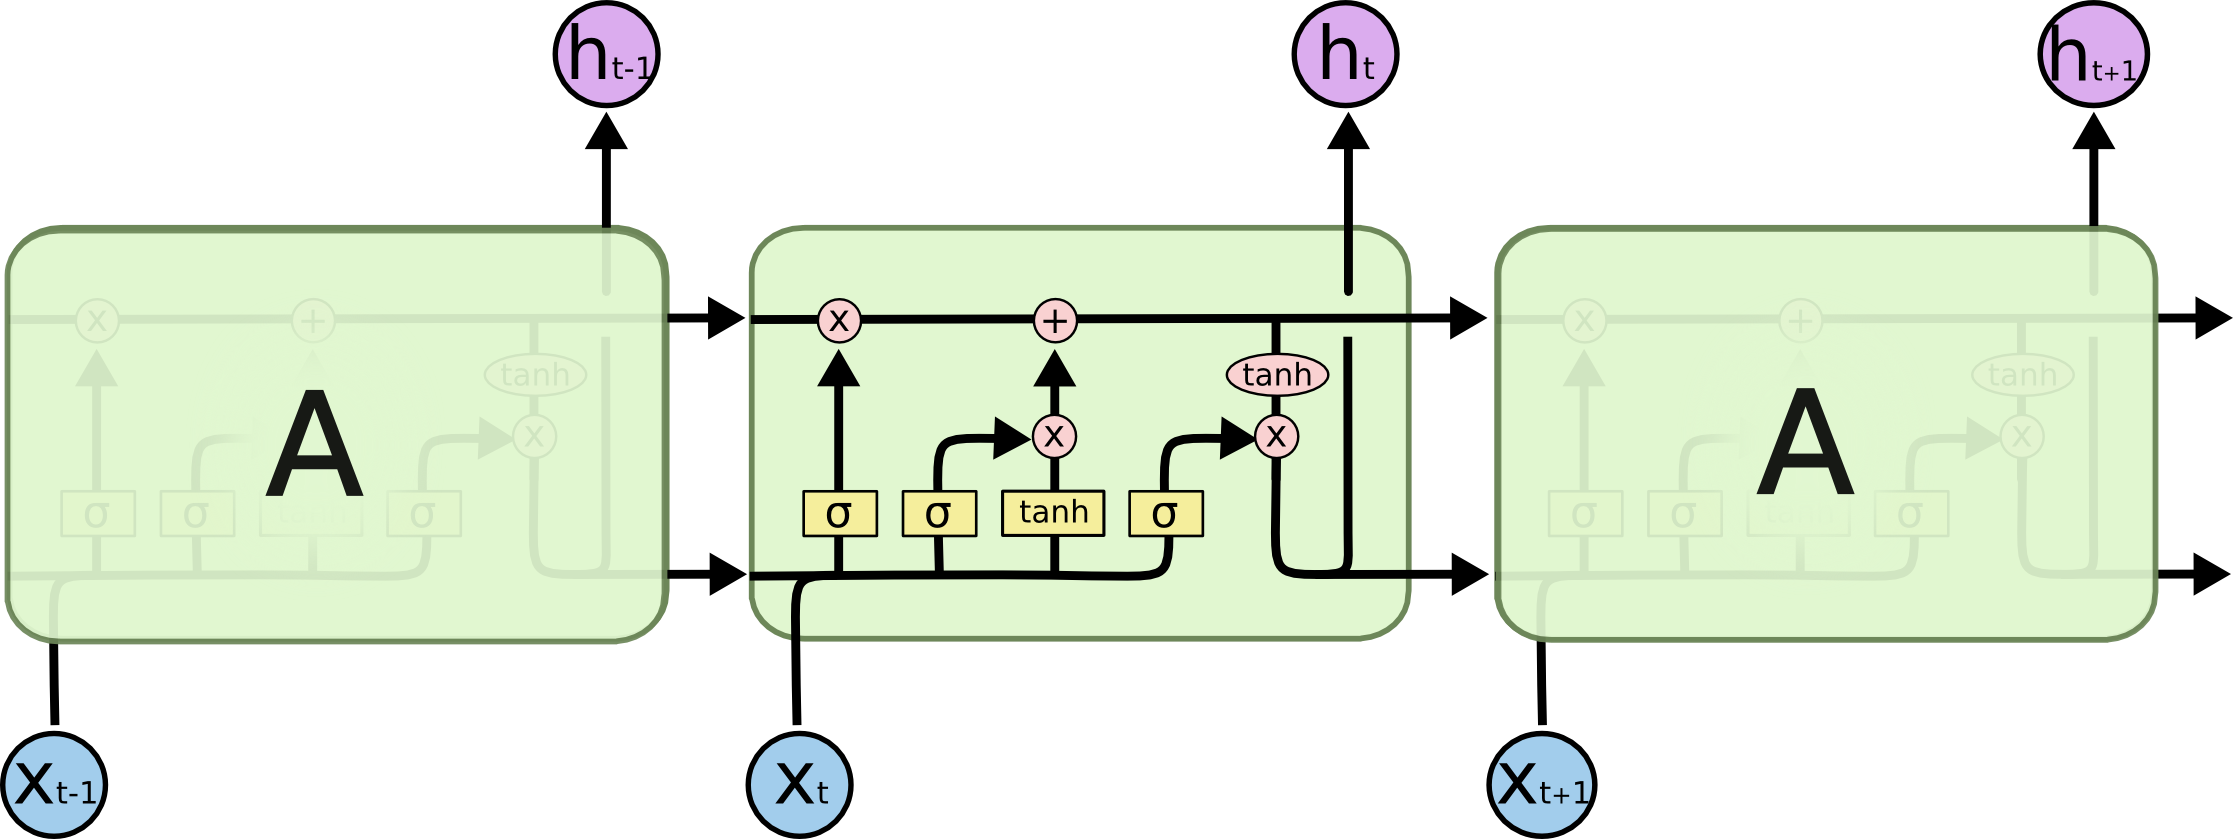
\includegraphics[width=0.6\textwidth]{Img/lstm.png}
    \bicaption{一个LSTM单元的结构表示。}{Illustration of an LSTM cell architecture.}
    \label{fig:lstm}
\end{figure}
其中,LSTM单元门的输出可以表示如下:
$$\begin{aligned}\left[\begin{array}{c}{{\mathbf{i}_{t}} \\ {\mathbf{f}_{t}} \\ \tilde{\mathrm{c}}_{t}} \\ {\mathbf{o}_{t}}\end{array}\right] &=\left[\begin{array}{c}{\sigma} \\ {\sigma} \\ {tanh} \\ {\sigma}\end{array}\right] \left( \mathbf{W} \left[\begin{array}{c}{\mathbf{x}_{t}} \\ {\mathbf{h}_{t-1}}\end{array}\right] +\mathbf{b} \right)  \tag{1} \\ \mathbf{c}_{t} &=\tilde{\mathbf{c}}_{t} \odot \mathbf{i}_{t}+\mathbf{c}_{t-1} \odot \mathbf{f}_{t} \tag{2} \\ \mathbf{h}_{t} &=\mathbf{o}_{t} \odot \tanh \left(\mathbf{c}_{t}\right) \tag{3} \end{aligned}$$
其中$\mathbf{x}_{t}$ 是在这个输入句子中的第$i^{th}$个token,$\mathbf{W}$是LSTM单元的权重矩阵,$\mathbf{b}$是偏置项,$\mathbf{\sigma}$是sigmod激活函数,$\mathbf{tanh}$是双曲正切函数,$\odot$是element-wise的乘法。
因此,BiLSTM最终可表示为 $h=[\overrightarrow{h}\oplus \overleftarrow{h}]$,其中 $ \overleftarrow{h}$ 和  $ \overleftarrow{h}$分别表示两层LSTM的输出, $\oplus$ 表示连接运算。
如图\ref{fig:bilstm}所示为BiLSTM的结构示意图。
\begin{figure}[htb]
    \centering
    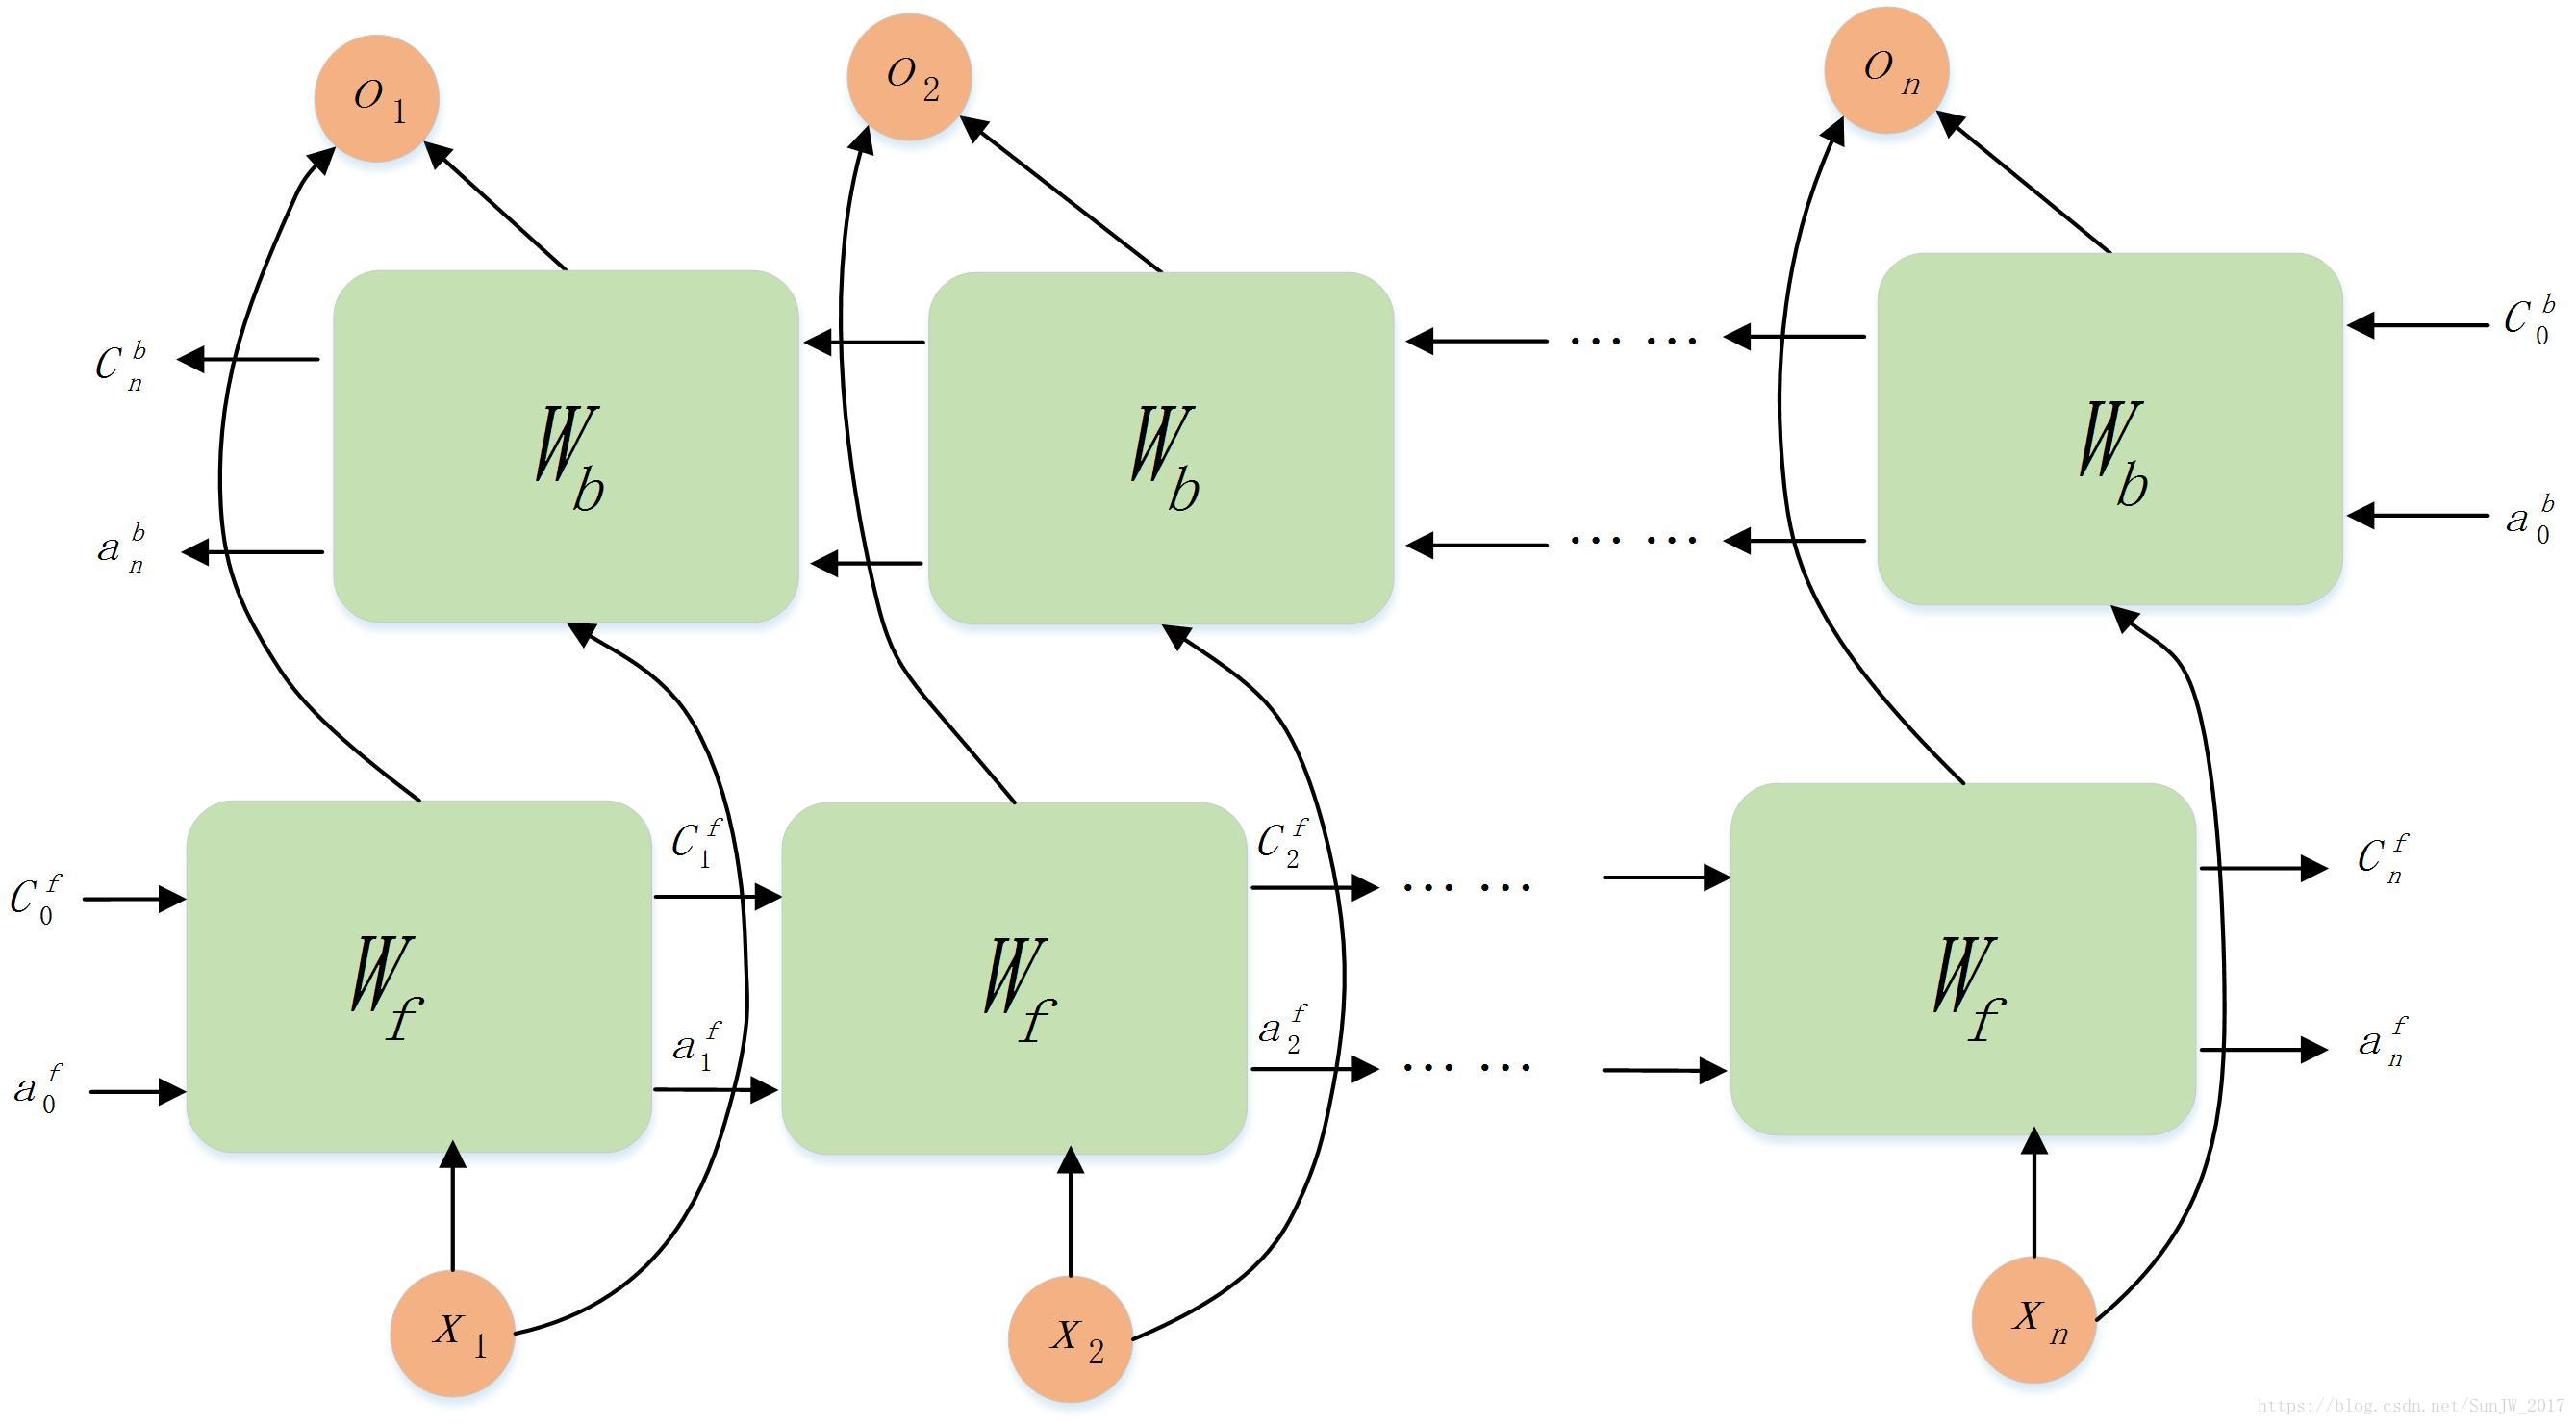
\includegraphics[width=0.6\textwidth]{Img/bilstm.jpg}
    \bicaption{BiLSTM的结构表示。}{Illustration of BiLSTM architecture.}
    \label{fig:bilstm}
\end{figure}

\subsection{文本分类模型}
朴素贝叶斯(Naive Bayesian)\cite{mccallum1998comparison}是基于词袋假设和贝叶斯公式的常用文本分类模型。对于文档$d$和类别$c$,该文档属于类别$c$的概率为$P(c|d)=\frac{P(d|c)P(c)}{P(d)}$,其极大后验也即最有可能的类别为$c_{MAP}=\mathop{\arg\max}\limits_{c \in C}P(c|d)$,去掉贝叶斯公式分母可得$c_{MAP}=\mathop{\arg\max}\limits_{c \in C}P(d|c)P(c)$,基于词袋模型和特征条件独立性假设可得
$$c_{NB}=\mathop{\arg\max}\limits_{c \in C}P(x_1|c)P(x_2|c)\dots P(x_n|c)P(c)=\mathop{\arg\max}\limits_{c \in C}p(c)\prod\limits_{x \in X}P(x|c)$$
因此,我们通过极大似然估计获得似然概率$P(x|c)$和先验概率$P(c)$即可得到后验概率$P(c|d)$,然后,我们将后验最大的类别作为分类结果。

fastText\cite{joulin2016bag}是Facebook开源的一个词向量计算和文本分类工具。
% ,其优点主要在于在文本分类任务中,fastText(浅层网络)往往能取得和深度网络相媲美的精度,却在训练时间上比深度网络快许多数量级。在标准的多核CPU上,能够在10分钟之内训练10亿词级别语料库的词向量,在1分钟之内能够分类有30多万类别的50多万条句子。
其模型架构和word2vec\cite{mikolov2013distributed}的CBOW模型架构非常相似,图\ref{fig:fasttext}所示为fastText的模型结构图。
\begin{figure}[htb]
    \centering
    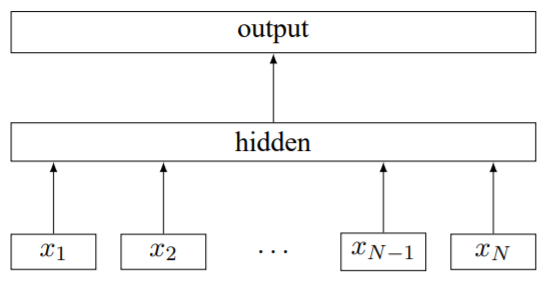
\includegraphics[width=0.6\textwidth]{Img/fastText.png}
    \bicaption{对于具有N ngram句子特征$x_1, \dots , x_N$ 的句子的fastText模型结构。特征被嵌入表示并且求平均来作为隐藏特征}{Model architecture of fastText for a sentence with N ngram features $x_1, \dots , x_N$ . The features are embedded and averaged to form the hidden variable}
    \label{fig:fasttext}
\end{figure}
fastText模型结构类似于CBOW只有三层,并且也利用了分层的Softmax减少训练时间。但是CBOW的输入是目标单词的上下文窗口,fastText的输入是用来表示单个文档的多个单词及其n-gram特征。CBOW的输出是目标词汇,fastText的输出是文档对应的类别。并且fastText将单词的字符级别的n-gram向量作为输入的额外特征。

随机森林(Random Forest)\cite{liaw2002classification}
随机森林是一种集成机器学习中Bagging的方法,其是由很多决策树构成的,不同决策树之间是独立的。当我们进行分类任务时,对于新的输入样本,森林中的每一棵决策树对其分别进行判断和分类,每个决策树会得到一个自己的分类结果,决策树的分类结果中哪一个分类最多,那么随机森林就会把这个结果当做最终的结果。它的构造过程首先对数据集合进行有放回的抽取,得到若干个子数据集,对于每个数据集中随机选取的特征,使用信息增益进行分裂,然后得到若干树组成森林。由于随机森林选取数据集和特征的随机性,其优点在于不容易过拟合,处理很高维度的数据,并且不用做特征选择,由于决策树并行生成,因此可以并行训练。

梯度提升决策树(Gradient Boosting Decision Tree)\cite{ke2017lightgbm}
梯度提升树是另一种基于树的集成机器学习方法,其模型定义为加法模型:
$$f_M(x)=\sum^M_{m=1}\alpha_mh_m(x,\theta_m)=\sum^M_{m=1}f(x,\theta_m)$$,其中$h_m$是第m棵树,$\alpha_m$是第m棵树的权重。GBDT目标函数为:
$$\large {r_{mi}} = -\left[\frac{\partial L(y_i,f(x_i))}{\partial f(x_i)} \right]_{f(x)=f_{m-1}(x)}$$,使用平法误差损失函数时$L(y, f(x)) = (y-f(x))^2$。其使用经验风险最小化求得下棵树的参数:
$$\hat \theta_{m} = \mathop{\arg\min}\limits_{\theta_{m}} \sum_{i=1}^ML(y_{i}, f_{m-1}(x_{i})+T(x_{i}; \theta_{m}))$$

\section{少样本学习}
深度学习在计算机视觉和NLP领域都取得了巨大的成功。但是它严重依赖于足够多的训练数据量,并且当标记的资源不足时,很难达到很好的效果。聊天消息中的自动挖掘技术还面临标注资源不足的问题。在在线聊天中,大量的开发人员会在短时间内创建大量讨论。为学习有效的模型标注大量的对话数据非常耗时,因为它们不仅文本很长,而且还需要领域知识来充分理解。于是少样本学习被提出来克服这些困难\cite{wang2019few}。少样本学习可以分为以下三类\cite{chen2019closer}:基于模型的方法:其旨在通过模型设计从少量标注数据的分类中学习映射函数;基于优化器的方法:其可调整传统的梯度下降优化器方法以拟合数据;基于度量的方法:其通过学习相似性度量函数对样本进行分类。
在本文中,我们利用了一种基于度量的少样本学习技术,即孪生网络\cite{bromley1994signature},该技术被广泛用于衡量文本或图像之间的语义相似性\cite{mueller2016siamese}。传统的分类模型尝试学习从单个实例映射到其类别的函数,但是当可用的标注资源数据较少时,它们不能达到理想的效果。与传统方法不同,孪生网络将成对的实例作为输入,旨在学习确定两个实例是属于同一类别还是属于不同类别的关键特征。它由两个相同的子模块组成,这些子模块不仅共享模型结构,而且还共享参数。从直觉上讲,对于本任务而言,确定两个对话是否相似而不是为每个对话指定确切的类别更容易。由于孪生网络将一对对话作为输入,因此数据集从元素级别转换为成对级别,并且可以通过排列组合进行数据增强。

\section{本章小结}

本章主要针对在构建我们提出的基于孪生网络从大规模聊天记录中进行需求对话识别的方法时涉及到的相关概念和关键技术进行详细调研和总结。其中基于文本数据的需求发现主要包括基于手工设计规则和基于统计机器学习的方法,它们在不同的数据来源包括issue tracker、邮件列表等取得了较好的效果;聊天对话文本目前被广泛运用在软件工程中,并被当作丰富的信息来源;从并行的多人、多轮对话中进行对话解耦是一项必不可缺的工作,目前基于神经网络的对话解耦取得了state-of-the-art的效果;在自然语言处理中,通常会通过TFIDF、GloVe等对对话文本进行嵌入式表示,并使用TexCNN等方法进行分本分类;针对对话数据标注困难、样本少的情况,我们介绍了当前常见的包括孪生网络等的少样本学习技术。

